\chapter{Introduction}

\textsl{The purpose of the current chapter is to describe the general characteristics of an AI enabled market research system, detail a list of aims and objectives, describe the adopted life cycle model, present a risk analysis and offer a project plan.}

\section{Problem Statement}
Marketing research is the systematic design, collection, analysis, and reporting of data related to the market of a company. When doing market research, most \ac{SME}s don’t know what to search for, struggle to find appropriate sources or lack the digital tools to properly analyse and make use of information. Nonetheless such data is vital for the success and functionality of businesses. For example, a company selling phones needs to see if the demand for mobile phones is growing or shrinking and know which accessories and phones are more popular and why. A physical restaurant should have a detailed knowledge of the dining trends of the food industry in their area. By interpreting historical data and deriving financial metrics from it such as pricing changes, sales growth, demand etc. \ac{SME}s can better understand the market they operate in, improve their competitiveness and make better decisions. Usually, large companies have their own complex systems for recording data, store it upon well-structured models, analyse it and generate useful reports. Such applications, however, are too expensive to build for \ac{SME}s and require lots of knowledge and data for their functionality to begin with \cite{digitaltrasformationsmes}. The purpose of this thesis is to build a \ac{MRS} that can aggregate market-related data from a variety of data sources (documents, logs, APIs, websites, online surveys etc.) and analyses it to generate useful information and data-driven marketing insights. Other \ac{MRS}s already exist, such as QuantCloud, a trading service that uses predictive algorithms to find patterns within stock market data and offer stock market insights \cite{quantcloud}. QuantCloud can calculate the seasonal volatility of log returns for grouped data, the Autoregressive-moving average (ARMA) etc. Another \ac{MRS} is Google Analytics which tracks websites usage and provides businesses with product trends, users behaviour information, custom reports etc. \cite{googleanalytics}. The mentioned systems all focus on very specific business problems. This thesis aims at building a general purpose \ac{MRS} that can offer an array of different metrics and that does not require specialized knowledge to be used. Marketing data usually display non-stationary behaviour, which means that the data points have dynamic means, variances, and covariances and they are affected by a number of implicit variables. Because of this non stationary data cannot be modelled well or forecasted accurately. This thesis wants to show how to analyse such data using kernel machines and unsupervised learning.

\section{Aims and Objectives}
The main goal of this project is to develop a prototype of a Web-based \ac{MRS} that leverages AI, ML and Big data technologies and that integrates and analyses data coming from different sources in order to produce marketing insights. In order to implement such a system, the following objectives have been set:
\begin{itemize}
	\item Implement a Search Module;
	\item Create an Aggregator module that fetches data from various sources and integrates it on a common model;
	\item Build an Analyser tool that performs data analysis using k-means and \ac{KRLS} methods;
	\item Build a data visualization dashboard;
	\item Configure a database to store, process and query existing market research data.
\end{itemize}

\newpage
\section{Life-cycle model}
For the implementation of the marketing research system the incremental model was used. The incremental model includes phases for tracing the progress of a product from a planned idea to its final release into operation and maintenance. The main characteristics of this life cycle approach are:

\begin{enumerate}  
	\item Architectural Analysis and Design activities are not repeated: the goal is to spend sufficient time studying the problem and gathering all the requirements so that the architecture of the system is can be fully identified during the initial stages of the project. This allows for a stronger planning;
	\item The implementation of the different parts of the system is incremental and is also planned in the initial stages of the project;
	\item The activities of Design, Coding and Verification are repeated in order to improve existing parts of the system, correct mistakes or add new features;
	\item Maintenance is a continuous activity and aims at making the product solid and bug free.
\end{enumerate}

The advantages of using this model are that the requirements are treated according to their strategic importance and the implementation starts from the primary ones. Furthermore, each increment adds new functionality to the baseline and allows any shareholder to test the application and give valuable feedback. Every successive iteration of the application should become more complete, converging to an appropriate final version of the product.

\begin{figure}[H]
	\centering
	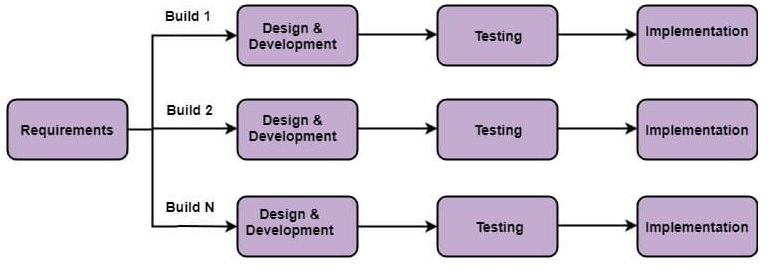
\includegraphics[scale=0.95]{img/incremental.jpg}
	\caption{Workflow of the incremental model, where a product is built incrementally.}
	\label{Introduction:Incremental Model}
\end{figure} 

\newpage
\section{Risks Analysis}
Every project is subject to risks. In order the manage them, the potential risks have been identified, the possible impact and consequences of each risk have been studied and preventive and corrective methods have been established:
\begin{itemize}
	\item Technological risks: depending on type of project, some tools might be better suited than others. Choosing the wrong tools is not particularly dangerous, but it can lead to wasting time, missing deadlines and having implementation and integration issues. In order to avoid this risk a longer period of time was allocated at the beginning to compare different tools according to project needs;
	\item Hardware failures: all the work is done using a laptop. Any problems with this device might have repercussions on the project. This is not very dangerous but it can lead to wasting time, missing deadlines and losing work. In order to account for this risk a second device is made available and the work is backed up regularly on remote repositories;
	\item Poor planning: this refers to a situation where the tasks to complete are not set out or are under or over estimated. This can be caused by a misunderstanding of the requirements or a deviation from the scope of the project. This can be dangerous and it can lead to wasting time, missing deadlines, unmet expectations and to the failure of the project. To account for this a longer period of time was allocated for the requirements analysis and the  literature Review and the \ac{CI/CD} method was used;
	\item Misunderstanding the requirements: sometimes business and technical professionals will not understand each other’s terminology and may have a different meaning for the same words. This can lead to misunderstanding the requirements. The danger of this happening is medium and it can lead to building the wrong product, wasting time and resources and safety issues. To avoid this risk longer time was spent in requirements analysis and the \ac{CI/CD} method was used;
	\item Conflicts with stakeholders: sometimes conflicts might arise between the different parties involved in a project. This can be extremely dangerous and it can result in the failure of the project. To avoid this it is necessary to decide all the important things at the beginning and make sure everyone is on the same page. 
\end{itemize}


\newpage
\section{Planning}

\begin{figure}[H]
	\centering
	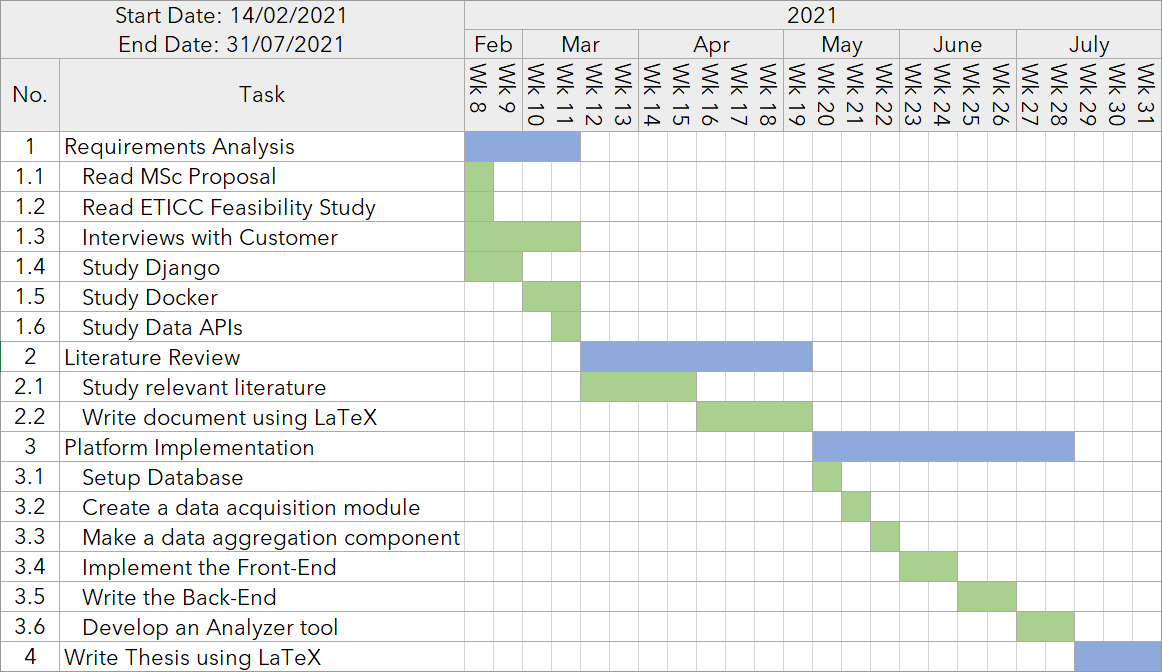
\includegraphics[scale=0.7]{img/gantt.png}
	\caption{The Gantt chart shows the activities involved in a project.}
	\label{Introduction:Gantt Chart}
\end{figure}

The activities and their subtasks have been scheduled using a Gantt chart, which is a useful tool for seeing the various dependencies between activities and sub-activities. In a Gantt chart is possible to represent, through black rhombuses, milestones that coincide with the end of a period or objectives to be achieved. The project started as part of an internship within a company located in Birmingham, but due to an unresolvable dispute over IP, the project was ultimately submitted under a different supervision. 








